\chapter{Security Implementations in OSI Levels}
\begin{quotebox-yellow}{}
    In the ISO/OSI stack, there is \textbf{not} a single optimal level in which we can implement security. Typically, L6 (Presentation) is the \textbf{only} level in which security measures are \textbf{not} useful.
\begin{itemize}
    \item The \textbf{higher} we go in the stack, the more our security features are \textbf{effective}, but we \textbf{slow}
    down our system and we leave more room for DoS attacks.
    \item The \textbf{lower} we go in the stack, the more \textbf{quickly} we detect attacks, but the \textbf{fewer} are he data available to us to detect them.
\end{itemize}
\end{quotebox-yellow}
\section{DHCP Security}
When L3 is reached, one of the first protocols that is activated is the \textbf{DHCP (Dynamic Host Configuration Protocol)}. Unfortunately, DHCP is \textbf{not} capable of performing peer authN
and uses \textbf{broadcast} packets that carry: IP address; netmask; default gateway; local DNS and local DNS suffix (\(\rightarrow \) \textbf{sensitive data}).\\   
\\    
Since DHCP Requests are L2 broadcast frames, an attacker could activate a \textbf{Fake DHCP
Server} by staying in the same broadcast domain of the victim and Sniffing the victim’s DHCP Request.\\    
\\    
Possible \textcolor{red}{\underline{\textbf{attacks}}} that can be performed by a Fake DHCP Server are:
\begin{itemize}
    \item \textbf{DoS}: done by providing a wrong network configuration to the victim, denying access to the network.
    \item \textbf{MIMT}:  a valid IP address is provided to the victim, but it will be a part of a /30 subnet (\(\rightarrow \) \textbf{only} two IP addresses can be assigned):
    \begin{itemize}
        \item One is given to the user
        \item The other is configured by the attacker as the victim’s default gateway
    \end{itemize}
    In this way, the victim is \textbf{ogically isolated} in a subnet of its own \(\rightarrow \) to communicate the victim has to send \textbf{everything} through the attacker.\\   
    \\
However, with this configuration, \textbf{incoming traffic} could still get to the victim \textbf{without} passing through the attacker. The attacker however could also activate NAT to successfully intercept the incoming traffic.
\item \textbf{Malicious Name-Address Translation}: the attacker declares himself as \textbf{Local DNS}. Then, when the victim wants to perform a \textbf{name} \(\rightarrow \) \textbf{address} translation, the attacker
will provide the wrong address. This tactic is usually used for Phishing and Pharming attacks;
\end{itemize}
CISCO tried to \textcolor{green}{\textbf{solve}} these security problems by implementing into switches: 
\begin{itemize}
    \item \textbf{DHCP Snooping}: the switch acepts \textbf{only} DHCP Reply from \textbf{trusted} ports.
    \item \textbf{IP Guard}: switching is performed \textbf{only} for IP addresses that have been issued from a
    \textbf{valid} DHCP Server.
\end{itemize}
\textcolor{red}{\textbf{N.B.}} There is a memory limit on how many valid IPs can be stored in the switch.
\subsection{AuthN for DHCP Messages}
\textbf{RFC-3118} uses HMAC-MD5 to perform \textbf{data authN} the DHCP Frames, but, given its complexity, it is rarely adopted: since HMAC is a Symmetric Protocol, a secret key needs to be installed \textbf{manually} on each machine that has to use DHCP and on each DHCP server. Moreover, since the key is Symmetric there is \textbf{no} way to distinguish between a DHCP Client and a DHCP Server.
\newpage
\section{VPN (Virtual Private Network)}
\begin{minipage}{0.6\textwidth}
%	\vspace{-0.5cm}
L3 is the first layer to provide \textbf{End-to-End Connectivity}, so it is possible to create both
\textbf{End-to-End Protection} and \textbf{VPN}s. End-to-End Protection is needed for \textbf{securing data} as soon as they exit from the node that has generated them, until they reach the final network interface. This means that the \textbf{only} possible attacks are those inside the node, allowing us to forget about all the other attacks that come from L3 (apart from DoS). 
\end{minipage} 
\hspace{0.3cm}
\begin{minipage}{0.4\textwidth}
    \centering
    \includegraphics[width=0.9\textwidth]{/home/lorenzo/Pictures/Screenshots/Screenshot from 2024-12-30 16-40-45.png}
\end{minipage}
\noindent
VPN is a technique (implemented via hardware and/or software) used to create a \textbf{Private Network} while using shared (possibly \textbf{untrusted}) channels and/or communication devices.
\begin{figure}[H]
    \centering
    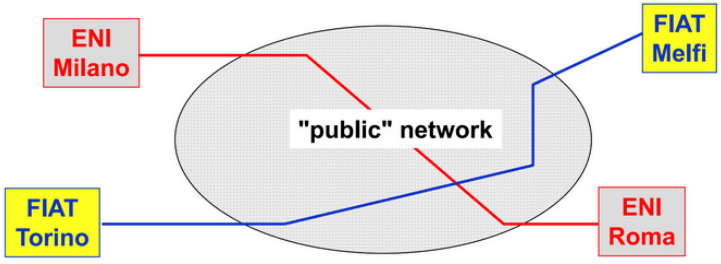
\includegraphics[width=0.5\textwidth]{/home/lorenzo/Notes/Information System Security/images/Screenshot from 2024-12-30 16-45-35.png}
    \caption{VPNs in a Public Network}
\end{figure}
A VPN can be created in three different ways:
\begin{itemize}
    \item \underline{\textbf{VPN via Private Address}}: The networks that want to be part of the VPN \textbf{must} use \textbf{Non-Public IP Addresses} that are \textbf{unreachable} from the other networks. These VPNs are considered \textbf{private} since they do not require authorization and the packets are \textbf{not} globally routable.\\   
    However, these protections can be easily defeated if somebody:
    \begin{itemize}
        \item Guesses or discovers the non-public IP addresses.
        \item Sniffs the packets during their transmission.
        \item Manages to access the communication devices.
    \end{itemize}
    \vspace{-0.2cm}
    \begin{quotebox-red}{Beware}
        This kind of VPN does not
        implement any type of protection for packets, users or the infrastructure itself \(\rightarrow \) the level of security of this solution is close to \textbf{zero}.
    \end{quotebox-red}
    \item \underline{\textbf{VPN via Tunnel}}: The routers encapsulate the whole L3 packet as the payload of another L3 packet (e.g. \textbf{IP in
    IP, IP over MPLS}, etc...). \textbf{Before} the encapsulation, the Border Routers perform \textbf{access} control to the VPN by checking an \textbf{ACL} (\textbf{Access Control List}).  
    For example, if the VPN belongs to the 10.1.0.0\textbackslash16 address range, the VPN can be accessed \textbf{only} by someone in 10.1.0.0\textbackslash16.\\    
    \\
    This solution grants VPN Providers protection against \textbf{malicious} VPN Customers, because it is impossible for Customers can change the subnet to which they belong (if they try, they do not belong anymore to the VPN).

    \begin{quotebox-red}{Beware}
        However, this protection can be defeated by anybody that \textbf{manages} a router or by Sniffing attacks \(\rightarrow \) protection works for Providers but \textbf{not} for Customers.
    \end{quotebox-red}
    \begin{quotebox-grey}{Example: VPN via IP Tunnel}
    \begin{minipage}{0.6\textwidth}
    %	\vspace{-0.5cm}
    \textbf{Net 1} and \textbf{Net 2} have got the \textbf{same color} because they belong to the \textbf{same subnet}.
    This VPN uses IP in IP Tunneling and works in the following way: 
    \begin{enumerate}
        \item \textbf{Node A} from \textbf{Net 1} sends a packet to \textbf{Node B} in \textbf{Net 2}.
        \item . The packet reaches the Border Router \textbf{R1}, which encapsulates it by adding the \textbf{IPv4 Header (Tunnel)}.
        \item The Tunneled Packet is forwarder from \textbf{R1} to \textbf{R2}.
        \item \textbf{R2} decapsulates the packet and forwards it to \textbf{Node 2}.
    \end{enumerate}
    \end{minipage} 
    \hspace{0.2cm}
    \begin{minipage}{0.4\textwidth}
        \centering
        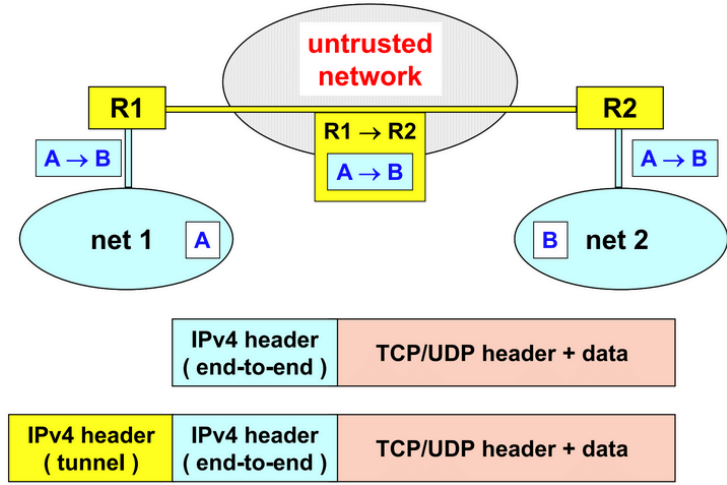
\includegraphics[width=0.9\textwidth]{/home/lorenzo/Notes/Information System Security/images/Screenshot from 2024-12-30 17-38-10.png}
    \end{minipage}
    \end{quotebox-grey}
    \item \underline{\textbf{VPN via Secure IP Tunnel}}: This type of VPN, also known as \textbf{S-VPN} (\textbf{Secure VP}), protects \textbf{also} VPN Customers. To
    do so, before encapsulation, the packets are protected with:
    \begin{itemize}
        \item \textbf{MAC}: grants \textbf{integrity} and \textbf{data authN}.
        \item \textbf{Encryption}: confidentiality.
        \item \textbf{Numbering}: to avoid Replay attacks.
    \end{itemize}
    There is \textbf{no} Digital Signature, because Asymmetric Encryption is \textbf{slow} and does \textbf{not} fit the
speed standards of modern networks. If the selected algorithms are \textbf{strong} \(\rightarrow \) only DoS attacks are possible.\\
\begin{minipage}{0.6\textwidth}
    %	\vspace{-0.5cm}
        In this picture, there are the Border Routers \textbf{R1} and \textbf{R2}, and the \textbf{TAP}s (\textbf{Tunnel Access Point}) \textbf{T1} and \textbf{T2}:
        \begin{itemize}
            \item Routers performs \textbf{encapsulation} and \textbf{decapsulatation}
            \item TAPs perform \textbf{cryptographic} and \textbf{decapsulatation}.
        \end{itemize}
    \end{minipage} 
    \hspace{0.2cm}
    \begin{minipage}{0.4\textwidth}
        \centering
        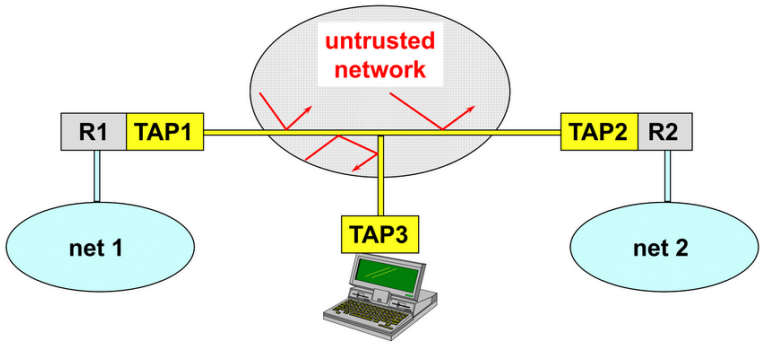
\includegraphics[width=0.9\textwidth]{/home/lorenzo/Notes/Information System Security/images/Screenshot from 2024-12-30 17-59-07.png}
    \end{minipage}
    \begin{quotebox-red}{Beware}
        If the TAP is managed by an \textbf{external} network Provider \(\rightarrow \) this is \textbf{fake security}.\\
        Security can be achieved only if there are separated devices, where:
        \begin{itemize}
            \item The TAPs are managed by the \textbf{client}.
            \item The Border Routers are be managed by the \textbf{ISP}.
        \end{itemize}
    \end{quotebox-red}
\end{itemize}
\noindent{\color{gray!50}\rule{\textwidth}{0.5pt}}
\section{IPsec}
IPSec (Internet Protocol Security) is a suite of protocols used to secure IP communications. It used to create:
\begin{itemize}
    \item \textbf{S-VPN} over \textbf{unstrusted} networks.
    \item \textbf{End-to-End secure packet flows}
\end{itemize}
IPsec defines two specific packet types:
\begin{itemize}
    \item \textbf{AH} (\textbf{Authentication Header}): provides \textbf{integrity}, \textbf{data authN} and protection against Replay attacks.
    \item \textbf{ESP} (\textbf{Encapsulating Security Payload}): provides nearly the same functions as \textbf{AH} and additionally grants \textbf{payload confidentiality}.\\    \\
    \textcolor{red}{\textbf{N.B.}} \textbf{Confidentiality} can \textbf{never} be provided for the \textbf{header}, if it is encrypted \(\rightarrow \) the intermediate systems would \textbf{not} be able to process the packets.
\end{itemize}
\noindent
Moreover, IPsec also defines \textbf{IKE} (\textbf{Internet Key Exchange}), which is a dedicated protocol for Key-Exchange.
\\ Thanks to all of these features, IPsec offers the following Security Services:
\begin{itemize}
    \item \textbf{AuthN of IP Packets}: achieved with the computation of a Keyed-Digest of the packets
    with a symmetric key. This provides:
    \begin{itemize}
        \item \textbf{Data Integrity}: the receiver can detect if the packets have been manipulated.
        \item \textbf{Sender AuthN}:  formal proof of the sender’s identity.
        \item \textbf{Partial} protection against Replay attacks \(\rightarrow \) working at L3 means that packets can be lost or duplicated.
    \end{itemize}
    \item \textbf{Confidentiality of IP Packets} \(\rightarrow \) but only for the \textbf{payload}.
    \item \textbf{Peer AuthN when Creating the SA}: when creating a \textbf{Security Association} (\textbf{SA}), a Key Agreement is needed \textbf{after} peer authN.
\end{itemize}

\subsection{SA (Security Association)}
A \textbf{SA} is an \textbf{unidirectional} logic connection between two IPsec systems. Each SA has associated a \textbf{single} and \textbf{unique} Security Service. To achieve \textbf{full protection} for a bidirectional
packet flow between two nodes, we \textbf{always} need two SAs, one A → B and one B → A.
\begin{figure}[H]
    \centering
    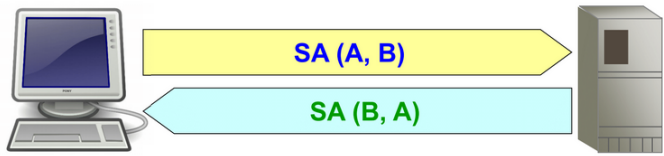
\includegraphics[width=0.5\textwidth]{/home/lorenzo/Notes/Information System Security/images/Screenshot from 2024-12-30 18-53-51.png}
\end{figure}

\subsection{Local "Database"}
SAs are managed via two \textbf{Local "Databases"}:
\begin{itemize}
    \item \textbf{SPD (Security Policy Database)}: contains the list of \textbf{Security Policies} (\textbf{SP}) to apply to different packet flows.
    The SPD is configured \textbf{a-priori} (e.g. manually) or connected to an \textbf{automatic system} (e.g. ISPS (Internet Security Policy System)).
    \item \textbf{SAD (SA Database)}:  a runtime "database" that contains a list of the \textbf{active} SAs and their characteristics (e.g. algorithms, keys, parameters).
\end{itemize}

\subsection{Sending Packet with IPsec}
When a node wants to send a packet and IPsec is installed on that node, the following questions need to be answered:
\\
\\
\begin{minipage}{0.6\textwidth}
%	\vspace{-0.5cm}
    \begin{itemize}
        \item Which SP should be applied to this packet? \(\rightarrow \) check the SPD:
        \begin{itemize}
            \item If a SP is provided \(\rightarrow \) it is applied
            \item If \textbf{no} SP is provided \(\rightarrow \)  the packet goes straight to L2 for transmission.
        \end{itemize}
        \item Is this the first packet of the flow? → check the SAD:
        \begin{itemize}
            \item If an SA is present \(\rightarrow \) IPsec applies the associated parameters that are used to
            protect the packet and then sends it to L2 for transmission.
            \item If \textbf{no} corresponding SA is present \(\rightarrow \) IPsec creates the corresponding SA and proceeds as above.
        \end{itemize}
    \end{itemize} 
\end{minipage} 
\hspace{0.3cm}
\begin{minipage}{0.4\textwidth}
    \centering
    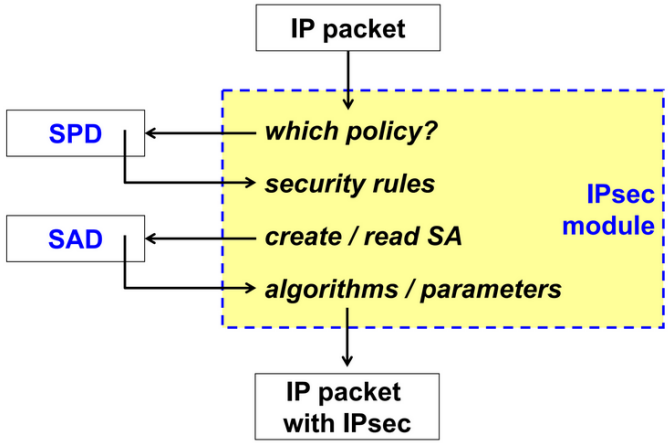
\includegraphics[width=0.9\textwidth]{/home/lorenzo/Notes/Information System Security/images/Screenshot from 2024-12-30 21-58-23.png}
\end{minipage}

\subsection{Transport Mode in IPsec}
\begin{minipage}{0.6\textwidth}
%	\vspace{-0.5cm}
Transport Mode is used for \textbf{End-to-End Security} by Hosts but \textbf{not} by Gateways.\\
The original packet is cut in two parts so that a new header (the \textbf{IPsec Header}) can be added
in between. The IPv4 header will say that it is transporting an IPsec Packet, while in the IPsec
Header there is a field that says what is the \textbf{actual} Transport Protocol (e.g. TCP, UDP) used
by the packet. 
\end{minipage} 
\hspace{0.3cm}
\begin{minipage}{0.4\textwidth}
    \centering
    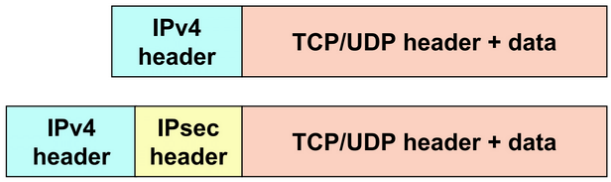
\includegraphics[width=\textwidth]{/home/lorenzo/Notes/Information System Security/images/Screenshot from 2024-12-30 22-03-48.png}
\end{minipage}
\begin{itemize}
    \item \textcolor{green}{\textbf{Pro}}: it is \textbf{fast}.
    \item \textcolor{red}{\textbf{Con}}: \textbf{no} protection of the IPv4 header. 
\end{itemize}

\subsection{Tunnel Mode in IPsec}
\begin{minipage}{0.6\textwidth}
%	\vspace{-0.5cm}
\textbf{Tunnel Mode} is used to create a VPN, usually, among Gateways.\\
In Tunnel Mode, the entire original IP packet, including \textbf{both the header and payload}, is encapsulated within a new IP packet. This provides \textbf{comprehensive protection} for the original packet, as encryption and authentication are applied to the encapsulated content.
Since the entire original IP packet (including the header) is encapsulated, all variable fields of
the inner header are fully protected, ensuring confidentiality and integrity (\textbf{Protection of End-to-End (E2E) Header Fields}). 
\end{minipage} 
\hspace{0.5cm}
\begin{minipage}{0.4\textwidth}
    \centering
    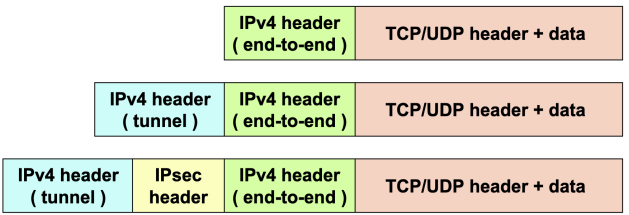
\includegraphics[width=\textwidth]{/home/lorenzo/Notes/Information System Security/images/Screenshot from 2024-12-30 22-18-55.png}
\end{minipage}

\begin{center}
\vspace{-0.4cm}
\begin{quotebox-red}{Beware}
    The Secure IPsec Tunnel is \textbf{not} created among Routers, but between the Gateways,
    since Gateways are the actual \textbf{contact point} between a secure network and an unsecure one
    \(\rightarrow \) the Gateway has the role of adding protection by creating a Secure IPsec Tunnel
\end{quotebox-red}
\end{center}
\begin{itemize}
    \item \textcolor{green}{\textbf{Pro}}: full packet confidentiality.
    \item \textcolor{red}{\textbf{Con}}: it is \textbf{slow}.
\end{itemize}
\newpage
\subsection{AH (Authentication Header)}
There are two version of \textbf{AH}:
\begin{itemize}
    \item \textbf{1v Version}: it provides \textbf{integrity} and \textbf{sender authN}. System who use this version
    \textbf{must} support \textbf{Keyed-MD5} and can \textbf{optionally} support \textbf{Keyed-SHA1}.
    \item \textbf{2v Version}: it provides \textbf{integrity}, \textbf{sender authN} and \textbf{partial} protection from Replay
    attacks. System who use this version \textbf{must} support \textbf{HMAC-MD5-96} and \textbf{HMAC-SHA1-96}.
\end{itemize}
The format of the header that is being added to the IPsec packet has:
\\    
\\
\begin{minipage}{0.6\textwidth}
%	\vspace{-0.5cm}
    \begin{itemize}
        \item \textbf{Next Header} (1 byte): it contains the real transporting protocol of the packet, since in the IP header there will be written that it is transporting AH.
        \item \textbf{Lenght} (1 byte): describes the length of the packet.
        \item \textbf{Reserved} (2 bytes): for future use.
        \item \textbf{SPI} (\textbf{Security Parameter Index}, 4 bytes): refer in a quick and easy way to all the parameters that are needed to protect the packet.
        \item \textbf{Sequence Number} (4 bytes): it is different from the one in the IP header, as it is used to avoid Replay attacks.
        \item \textbf{ICV} (\textbf{Integrity Check Value}): Digest that provides \textbf{data authN}.
    \end{itemize}
\end{minipage} 
\hspace{0.3cm}
\begin{minipage}{0.4\textwidth}
    \centering
    \includegraphics[width=1\textwidth]{/home/lorenzo/Pictures/Screenshots/Screenshot from 2024-12-30 22-34-23.png}
\end{minipage}
\\  
\\   
\\
\noindent
\begin{minipage}{0.6\textwidth}
%	\vspace{-0.5cm}
Once an IPsec packet with AH Header has been received, the ICV is extracted. Meanwhile the whole packet is normalized, in order to put the packet in the same conditions as it was at the sender in order to correctly compute the Digest. The SPI is also extracted from the AH header to get the correct entry from the SAD, which contains the correct parameters needed to compute the Digest.\\
\\
\textbf{After} having computed the Digest of the normalized packet, it is compared with the extracted
ICV:
\begin{itemize}
    \item If the values are the same \(\rightarrow \) the Sender is authN and the integrity of the packet is
    confirmed.
    \item If the values are \textbf{not} the same \(\rightarrow \) the sender is \textbf{not} authN and/or the packet has been manipulated;
\end{itemize} 
\end{minipage} 
\hspace{0.3cm}
\begin{minipage}{0.4\textwidth}
    \centering
    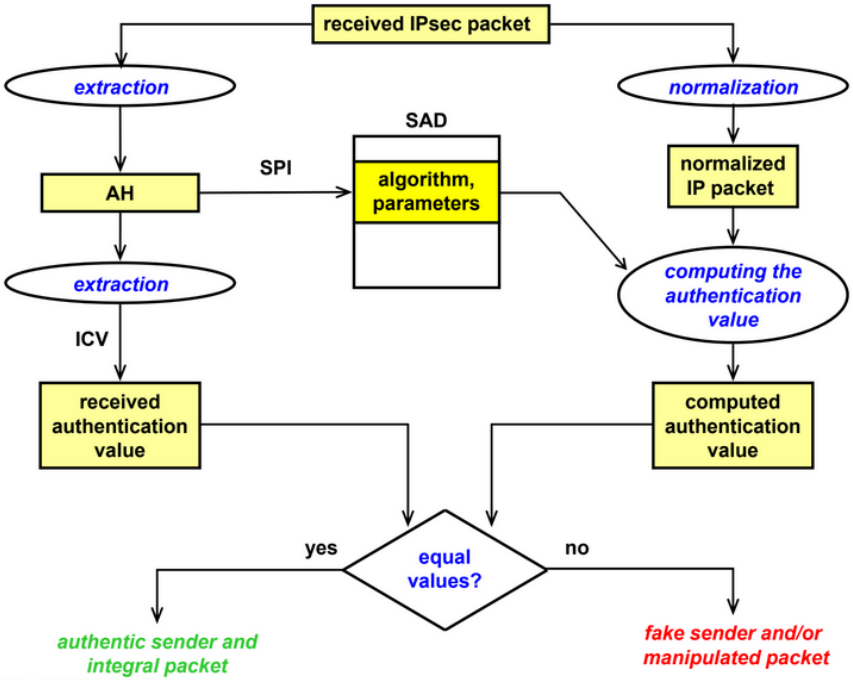
\includegraphics[width=\textwidth]{/home/lorenzo/Notes/Information System Security/images/Screenshot from 2024-12-30 22-43-13.png}
\end{minipage}
\\    
\\
\\
\noindent
\textbf{Sender authN} is guaranteed by the fact that the SA in the SAD has been implicitly arranged with the sender node. Thus, real authN comes into play when we create the SA.

\subsection{ESP (Encapsulating Security Payload)}
If AH’s security properties are \textbf{not} enough and we want \textbf{confidentiality} \(\rightarrow \) \textbf{ESP} is needed.\\
As AH, ESP comes in two versions:
\begin{itemize}
    \item \textbf{v1 Version}: it achieves \textbf{only confidentiality} using \textbf{DES-CBC}.
    \item \textbf{v2 Version}: it provides also \textbf{payload authN}. The \textbf{advantage} is that the packet dimension is \textbf{reduced} and \textbf{only} one SA is saved.
\end{itemize}
\textcolor{red}{\textbf{N.B.}}  IPsec’s architecture allows us to use AH and ESP at the same time, if needed.
\\
\\
ESP can be used in two modes:
\begin{itemize}
    \begin{minipage}{0.6\textwidth}
    \vspace{0.2cm}
    \item \textbf{Transport Mode}: The \textbf{ESP Header} is inserted in \textbf{between} the IPv4 Header and the Payload, while the \textbf{ESP Trailer} is \textbf{appended} at the end of the whole packet. Finally, \textbf{everything}, from the ESP header up to the trailer, gets then \textbf{encrypted}. 
    \begin{itemize}
        \item \textcolor{green}{\textbf{Pro}}: the payload is hidden.
        \item \textcolor{red}{\textbf{Con}}: the IP Header remains in clear. 
    \end{itemize}
    \end{minipage} 
    \hspace{0.0cm}
    \begin{minipage}{0.4\textwidth}
        \centering
        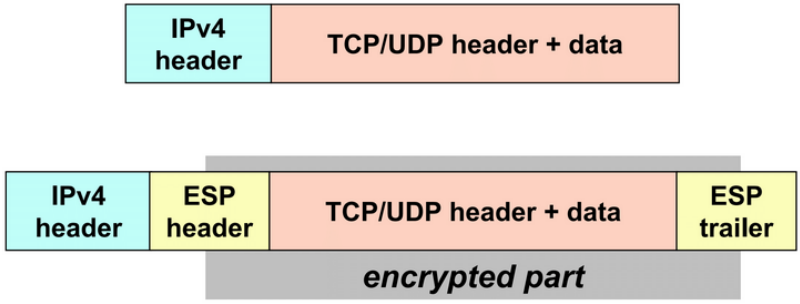
\includegraphics[width=0.8\textwidth]{/home/lorenzo/Notes/Information System Security/images/Screenshot from 2024-12-30 23-01-28.png}
    \end{minipage}

    \begin{minipage}{0.6\textwidth}
    %	\vspace{-0.5cm}
    \item \textbf{Tunnel Mode}: The first Tunnel is created, then the \textbf{ESP Header} is inserted in between the \textbf{IPv4 Tunnel Header} and the \textbf{IPv4 End-to-End Header}, while the \textbf{ESP Trailer} is appended at the end of the whole packet. As in Transport Mode, \textbf{everything}, from the ESP header up to the
    trailer, gets then \textbf{encrypted}.
    \begin{itemize}
        \item \textcolor{green}{\textbf{Pro}}: the original  Header and the Payload are \textbf{hidden}.
        \item \textcolor{red}{\textbf{Con}}: \textbf{larger}packet size.
    \end{itemize}
    \end{minipage} 
    \hspace{0.0cm}
    \begin{minipage}{0.4\textwidth}
        \centering
        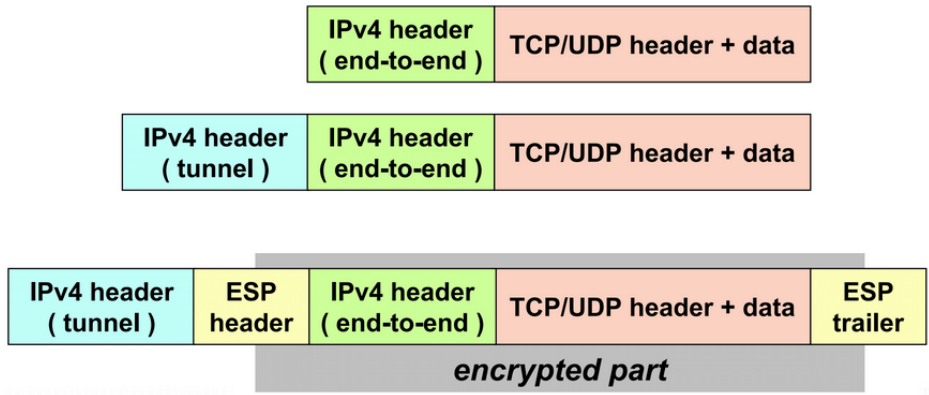
\includegraphics[width=0.8\textwidth]{/home/lorenzo/Notes/Information System Security/images/Screenshot from 2024-12-30 23-09-37.png}
    \end{minipage}
\end{itemize}

\subsection{IPsec Implementation Details}
Many algorithms can be used to implement IPsec, thus two main Crypto-Suites were defined to implement it:
\begin{itemize}
    \item \textbf{VPN-A}: uses \textbf{ESP} with \textbf{3DES-CBC} and \textbf{HMAC-SHA1-96}, this is a kind of \textbf{legacy
    VPN} for compatibility with old systems \(\rightarrow \) less secure.
    \item \textbf{VPN-B}: uses \textbf{ESP} with \textbf{ES-128-CBC} and \textbf{AES-XCBC-MAC-96}, which is the one used in modern systems \(\rightarrow \) more secure.
\end{itemize}
ESP adds also the possibility to use \textbf{NULL Algorithms}, where it is possible to specify \textbf{NULL}
for one of the two parts (authN or confidentiality), but \textbf{not simultaneously} \(\rightarrow \) "protection
against performance" trade-off.

\begin{center}
    \begin{quotebox-grey}{IPsec Partial Protection Against Replay Attacks}
        ESP’s and AH’s \textbf{Sequence Number} provide \textbf{partial} protection from replay attacks since it
        means that IPsec works with a minimum window of 32 packets (64 is the suggested one).\\    \\
        When the SA is created, the sender initializes the Sequence Number to 0. Every time a packet
        is sent, the Sequence Number is incremented by one, and once the value \(2^{31}-1\) is reached, a new SA should be negotiated. The window moves as valid packets are received \(\rightarrow \) \textbf{outside} the window, there is \textbf{no} protection against replay attacks.
      
            \centering
            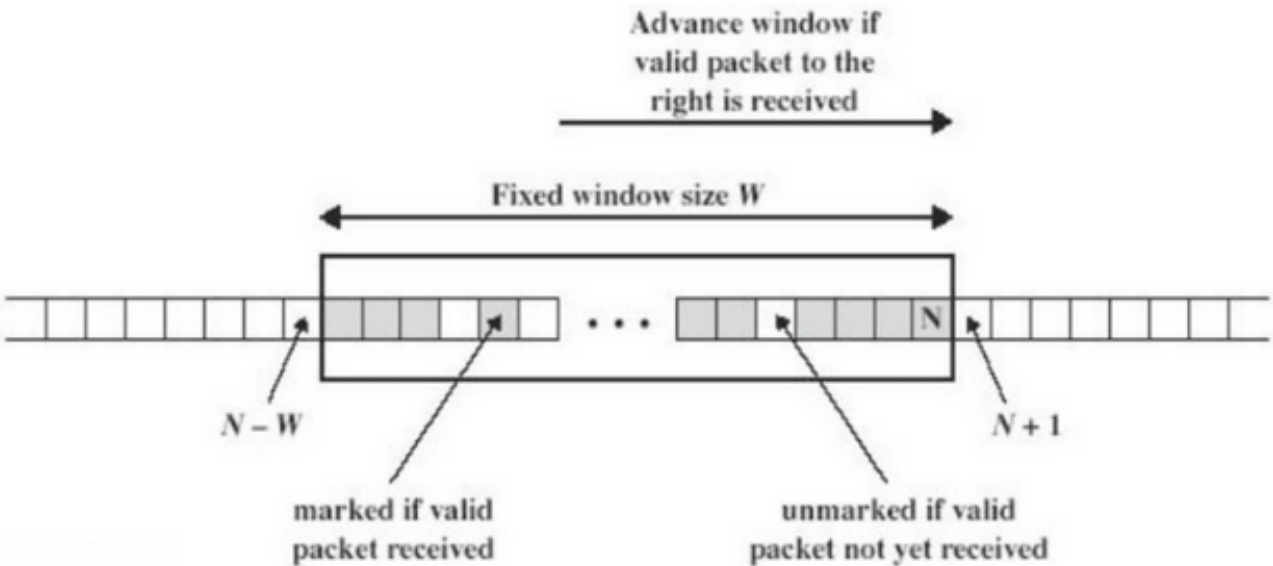
\includegraphics[width=0.5\textwidth]{/home/lorenzo/Notes/Information System Security/images/image copy 24.png}
    \end{quotebox-grey}   
\end{center}

\subsection{IPsec v3}
\textbf{IPsec v3} makes \textbf{ESP mandatory} and \textbf{AH optional}. It also adds support for single source
multicast. Moreover, to avoid overflow in highly trafficked channels, the \textbf{ESN} (\textbf{Extended Sequence Number}) has been introduced. It uses 8 bytes even though packets inside it are
still 4 bytes \textbf{only}, because \textbf{only} the 4 LSBytes transmitted (default with \textbf{IKEv2}). Finally, v3 adds support for AEAD and clarifies things about SA and SPI to manage faster lookup. The algorithms used in IPsec v3 are the following:
\begin{itemize}
    \item For \textbf{integrity} and \textbf{authN}:
    \begin{itemize}
        \item We may use \textbf{HMAC-MD5-96}.
        \item We must use \textbf{HMAC-SHA1-96}.
        \item We should use \textbf{AES-XCBC-MAC-96}.
        \item We \textbf{must} use \textbf{NULL}, but only if \textbf{ESP} is used.
        \item For a longer digest, we may use:
        \begin{itemize}
            \item \textbf{HMAC-SHA256-128}
            \item \textbf{HMAC-SHA384-192}
            \item \textbf{HMAC-SHA512-256}
        \end{itemize}
    \end{itemize}
    \item For \textbf{privacy}:
    \begin{itemize}
        \item We must use NULL;
        \item We must not use 3DES-CBC;
        \item We should use AES-128-CBC;
        \item We may use AES-CTR;
        \item We should not use DES-CBC;
    \end{itemize}
    \item For \textbf{authN encryption} in \textbf{AEAD Mode} (see below), we can use:
    \begin{itemize}
        \item \textbf{HMAC-SHA256-128}
        \item \textbf{HMAC-SHA384-192}
        \item \textbf{HMAC-SHA512-256}
    \end{itemize}
\end{itemize}
\begin{quotebox}[colframe=blue!10!white, colback=blue!5!white]{TFC (Traffic Flow Confidentiality)}
    \textbf{TFC} is a \textbf{padding technique} used in ESP that puts padding \textbf{after} the payload and before
    the normal padding: this is needed in order to \textbf{not} disclose what is the \textbf{real size} of the payload in the packet.\\     \\    
    Thanks to the length fields (e.g. in TCP, UDP, etc...) the receiver is able to compute the \textbf{original} size of the payload.\\     \\  
    \textbf{Dummy Packets} are a form of Nested Pseudo-Protocol that is introduced by IPsec v3 to keep
    transmitting even in \textbf{absence} of real data to send, which is essential to keep \textbf{confidentiality}.
    Even the Dummy Packets \textbf{must} be encrypted, in order to make them \textbf{indistinguishable} from
    real traffic.
\end{quotebox}

\subsection{Ways to use IPsec}
IPsec can be used to implement various security models:
\begin{itemize}
    \item 
\end{itemize}